% --------------- PLANTILLA MAXI (GOD) -----------------
\documentclass[11pt, twocolumn]{article}

\usepackage[latin1,utf8]{inputenc}
\usepackage{verbatim}
\usepackage{multirow}
\usepackage{float}
\usepackage{enumerate}
\usepackage{graphics,graphicx,xcolor}
\usepackage{subfig}
\usepackage[spanish,es-tabla]{babel}
\usepackage{caption}
\usepackage{placeins}
\usepackage{afterpage}
\usepackage{blindtext}
\usepackage{multicol}
\usepackage{geometry}
\usepackage{lipsum}

%paquete para referencias
\usepackage[backend=biber, style=nature, citestyle=numeric, sorting=none, maxbibnames=99]{biblatex} % 
% \usepackage{natbib}
% \bibliographystyle{apsrev4-1} % Utiliza el archivo .bst de APS o uno similar

\usepackage{titling} % Paquete para personalizar título del documento
\usepackage{authblk}  % Paquete para personalizar autores del documento
\renewcommand\Authand{ y } % Reemplazar 'and' con 'y'

\DeclareCaptionFormat{custom}
{%
    \textbf{#1#2}\textit{\small #3}
}
\captionsetup{format=custom}

\newgeometry{bottom=3cm, top=2cm, left=3cm, right=3cm}
\usepackage{hyperref}
\hypersetup{
  colorlinks   = true, %Colours links instead of ugly boxes
  urlcolor     = blue, %Colour for external hyperlinks
  linkcolor    = black, %Colour of internal links
  citecolor   = black %Colour of citations
}

%paquete para unidades
\usepackage{siunitx}
% seteo punto como separador decimal
\AtBeginDocument{\decimalpoint}


% \DeclareSIUnit\torr{Torr}

%% Paquetes de la AMS
\usepackage{amsmath, amsthm, amsfonts, amssymb}

%componentes de texto
\usepackage{textcomp}


% Personaliza título del documento
\pretitle{\begin{center}\LARGE\bfseries}
    \posttitle{\par\vspace{0.5em}\end{center}\large}
    \preauthor{\begin{center}\large \lineskip 0.8em \begin{tabular}[t]{c}}
    \postauthor{\end{tabular}\par\end{center}}
    \predate{\begin{center}\large}
    \postdate{\par\end{center}}


\usepackage{fancyhdr}
\pagestyle{fancy}

% Definimos el encabezado de las paginas pares e impares.
\lhead{REDES NEURONALES}
\chead{Práctica 4 - 2024}
\rhead{Gatto Maximiliano}
\renewcommand{\headrulewidth}{0.5pt}

% aqui definimos el pie de pagina de las paginas pares e impares.
\lfoot[a1]{}
\cfoot[c1]{\thepage}
\rfoot[e1]{}

\renewcommand{\footrulewidth}{0.5pt}

% ------------------- TITULO ----------------------
\title{{\large REDES NEURONALES - PRÁCTICA 4 - 2024} \\ \vspace{1cm}\textbf{Aprendizaje supervisado en redes multicapas}}



\author[ ]{\textbf{Maximiliano Gatto}}
\affil[ ]{Instituto Balseiro (UNCuyo - CNEA) - Bariloche, Río Negro, Argentina\vspace{0.4cm}}
\affil[ ]{\href{mailto:maximiliano.gatto@ib.edu.ar}{maximiliano.gatto@ib.edu.ar}}

\date{\today}

\begin{document}
\maketitle

% ------------------ INTRODUCCION ---------------------
\section{Introducción}

En esta práctica se analizaron distintas arquitecturas de redes neuronales para resolver diversos problemas algorítmicos. Para el entrenamiento de las redes, se implementó el algoritmo de retropropagación de errores (\textit{backpropagation}). Se establecieron métricas clave para evaluar el rendimiento de las redes, y se emplearon para compararlas entre sí. Todos los ejercicios fueron implementados mediante un script en \texttt{Python}, cuyo código está disponible en este \href{https://github.com/elmasi2393/Redes-neuronales/tree/main}{enlace}.


% ------------------ RESULTADOS ---------------------
\section{Resultados}

% --------------- EJERCICIO 1 ---------------------
\subsection*{Ejercicio 1}
En este ejercicio, se implementaron dos arquitecturas de redes neuronales (ver Figura \ref{fig:arquitecturas}) para resolver el problema de una compuerta XOR de 2 entradas, donde cada entrada puede tomar valores \(\pm 1\). La salida es \(-1\) si ambas entradas son iguales y \(1\) si son diferentes. Se utilizó la función de activación \(\tanh(x)\) con umbrales (\textit{bias}). El entrenamiento de cada red se realizó con el algoritmo de retropropagación de errores (\textit{backpropagation}) durante 2000 épocas, con una tasa de aprendizaje (\textit{learning rate}) de \(lr = 0.1\).

\begin{figure} [htbp]
  \centering
  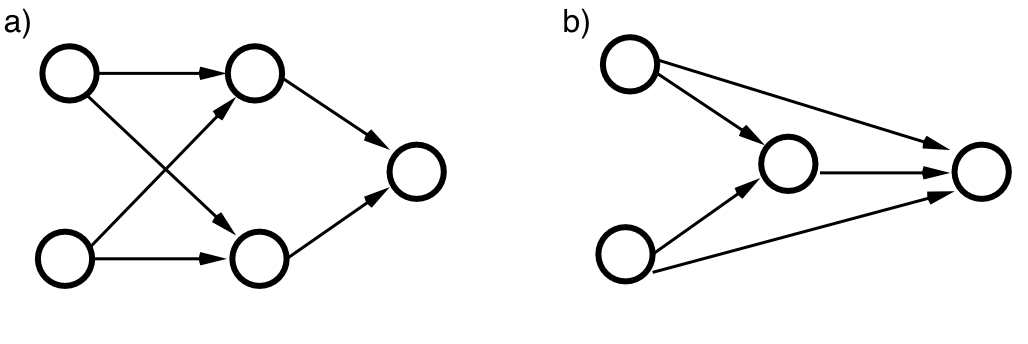
\includegraphics[width=0.45\textwidth]{figures/arquitecturas.png}
  \caption{(a) arquitectura 1, (b) arquitectura 2}
  \label{fig:arquitecturas}
\end{figure}


Para analizar la convergencia del algoritmo, se implementaron dos métricas. La primera es la \textit{accuracy} o precisión, que mide cuán bien la red clasifica las instancias de un conjunto de datos. Se calcula como:

\begin{equation} \label{eq:accuracy_discreto}
  \text{accuracy} = \frac{N^\circ \text{pred. correctas}}{N^\circ \text{pred. totales}} * 100,
\end{equation}

\noindent es decir, el porcentaje de instancias clasificadas correctamente sobre el total. Esta definición (Ecuación \ref{eq:accuracy_discreto}) se aplica a redes con salidas discretas. En nuestro caso, como la salida es continua, consideramos una predicción correcta si \(|y - o| < \epsilon\), donde \(y\) es la salida deseada, \(o\) es la salida de la red, y \(\epsilon\) es una constante pequeña, con un valor de \(\epsilon = 0.1\) en este trabajo.

La segunda métrica utilizada es el error cuadrático medio (MSE, \textit{mean squared error}), definido como:

\begin{equation} \label{eq:mse}
  \text{MSE} = \frac{1}{N} \sum_{i=1}^N (y_i - o_i)^2,
\end{equation}

donde \(N\) es el número de ejemplos de entrenamiento. Un MSE (Ecuación \ref{eq:mse}) más bajo indica que las predicciones son más cercanas a los valores reales.

Se analizó el tiempo medio de convergencia de ambas arquitecturas tras 10 condiciones iniciales aleatorias, considerando como convergencia la época en que \(\text{MSE} < 0.01\). El tiempo medio es el promedio de cada sorteo. La Figura \ref{fig:metrics_e1} muestra la evolución del accuracy y el MSE para cada arquitectura.

\begin{figure}[htbp]
  \centering
  \subfloat[]{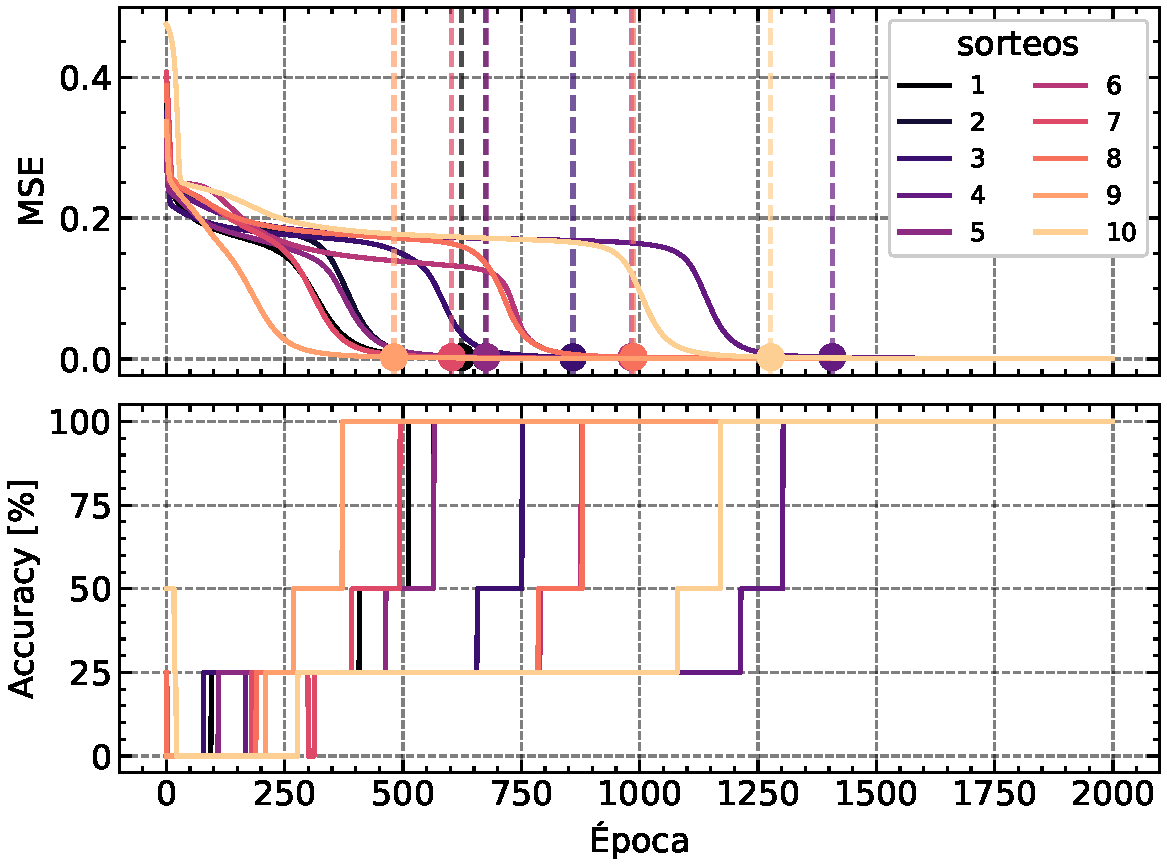
\includegraphics[width=0.45\textwidth]{figures/metrics_e1_1.pdf}\label{fig:mse_detec}}
  \hfill
  \subfloat[]{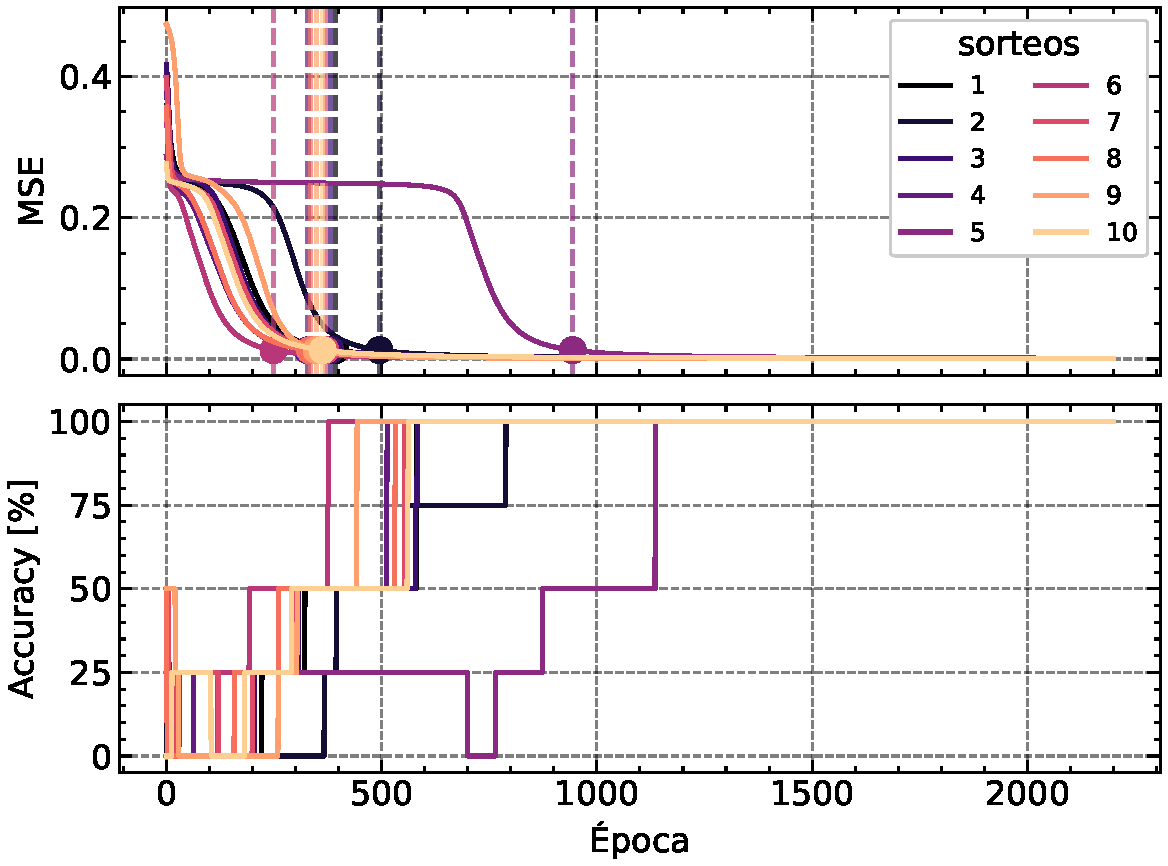
\includegraphics[width=0.45\textwidth]{figures/metrics_e1_2.pdf}\label{fig:psnr_detec}}
  \hfill
  \caption{métricas obtenidas durante el entrenamiento para diferentes sorteos de condiciones iniciales. El punto y la línea de trazos representa la época en la cuál se considera la convergencia. (a) arquitectura 1 y (b) arquitectura 2.}
  \label{fig:metrics_e1}
\end{figure}

%  Arquitectura 1: Mean convergence time: 857.1 +- 28.951906672963702
% Arquitectura 2: Mean convergence time: 420.5 +- 18.39327322691641

Como resultado, se obtuvo que la arquitectura 1 tiene un tiempo medio de convergencia de \(860(30)\) épocas, mientras que la arquitectura 2 converge en promedio en \(420(20)\) épocas. Por lo tanto, el resultado que se obtuvo es que la arquitectura 2 converge en promedio más rápido. Sin embargo,e ste resultado depende de la semilla inicial que se establece en el sorteo.

% --------------- EJERCICIO 2 ---------------------
\subsection*{Ejercicio 2}
% En este ejercicio se implementó una red como la de la Figura \ref{fig:arquitectura_e2} para resolver el problema de la paridad. Se trata de una generalización del XOR para N entradas, en donde la salida es 1 si el producto de las N entradas es 1, y \(-1\) si el producto es \(-1\).

En este ejercicio se implementó una red, como la de la Figura \ref{fig:arquitectura_e2}, para resolver el problema de la paridad, una generalización del XOR para \(N\) entradas. La salida es \(1\) si el producto de las entradas es \(1\) y \(-1\) si es \(-1\).


\begin{figure} [htbp]
  \centering
  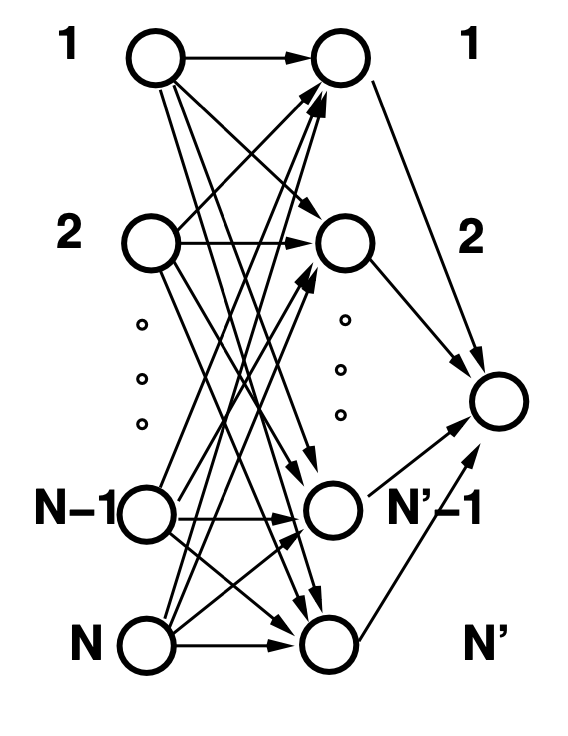
\includegraphics[width=0.25\textwidth]{figures/arquitectura e2.png}
  \caption{arquitectura del ejercicio 2 para resolver el problema de la paridad.}
  \label{fig:arquitectura_e2}
\end{figure}

Las redes fueron entrenadas con el algoritmo de retropropagación durante 40000 épocas, usando una tasa de aprendizaje (\(lr = 0.1\)) con \(N = 5\) entradas y variando el número de neuronas en la capa oculta (\(N' = 1, 3, 6, 7, 9, 11\)). Para evaluar el desempeño, se calcularon el \textit{accuracy} y el error cuadrático medio (MSE). Los resultados se presentan en la Figura \ref{fig:metrics_e2}.

\begin{figure} [htbp]
  \centering
  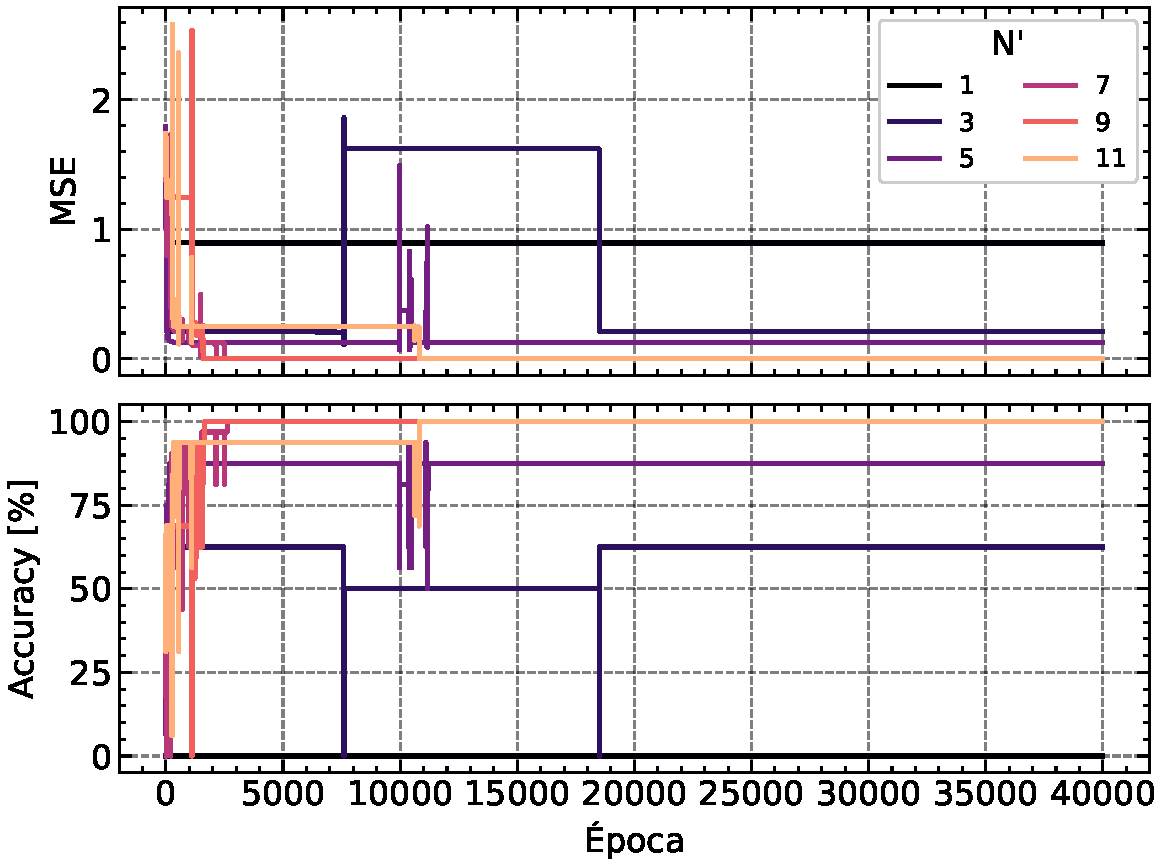
\includegraphics[width=0.45\textwidth]{figures/metrics_e2.pdf}
  \caption{métricas obtenidas durante el entrenamiento para diferentes valores de la capa oculta en la arquitectura del ejercicio 2.}
  \label{fig:metrics_e2}
\end{figure}

La Figura \ref{fig:metrics_e2} muestra que cuando \(N' < N\), el MSE es más alto y el accuracy no alcanza el 100\% (logrado por el epsilon en el conteo de predicciones correctas). En particular, con \(N' = 1\), la red no aprendió el algoritmo correctamente. El error disminuye y el accuracy mejora a medida que \(N'\) se acerca a \(N\). Para \(N' > N\), tanto el MSE como el accuracy son similares, indicando que la red puede resolver el problema de paridad, mientras que con \(N' < N\), el desempeño es peor y empeora a medida que \(N'\) disminuye.


% --------------- EJERCICIO 3 ---------------------
\subsection*{Ejercicio 3}
Se implementó una red neuronal, según la arquitectura de la Figura \ref{fig:arquitectura_e3}, para aprender el mapeo logístico \(x(t+1) = 4 x(t) (1 - x(t))\) mediante el algoritmo de retropropagación. La capa oculta utilizó la función de activación sigmoide \(g(x) = 1 / (1 + \exp(-x))\), y la neurona de salida una función lineal. La red contaba con umbrales y 5 neuronas en la capa oculta. El entrenamiento se realizó en 500 iteraciones utilizando el paquete \texttt{TensorFlow}.

\begin{figure} [htbp]
  \centering
  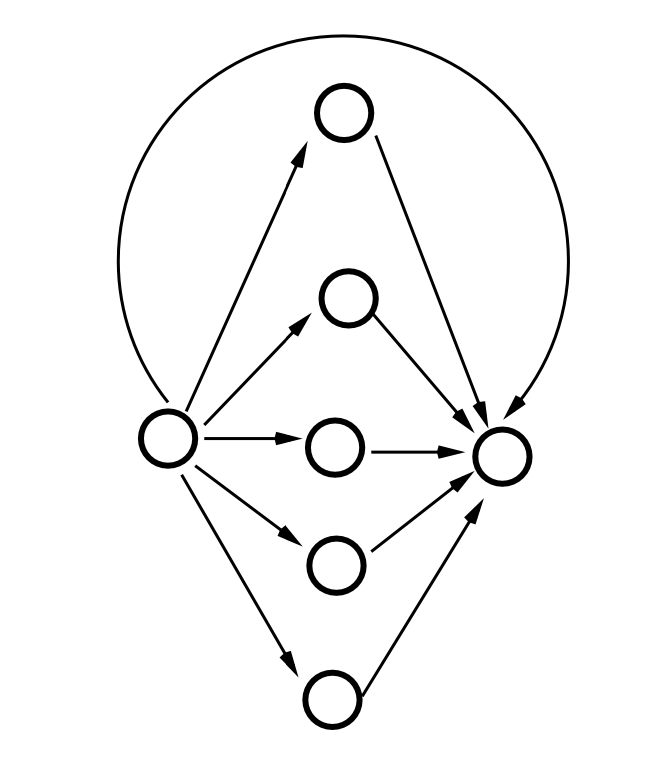
\includegraphics[width=0.25\textwidth]{figures/arquitectura_e3.png}
  \caption{arquitectura del ejercicio 3 para aprender el mapeo logístico.}
  \label{fig:arquitectura_e3}
\end{figure}

Se generaron aleatoriamente los valores de \(x(t)\) y se aplicó la regla de selección. Se evaluó el desempeño de la red con 5, 10 y 100 ejemplos de entrenamiento, comparando el error de entrenamiento y el de generalización. Los resultados se presentan en la Figura \ref{fig:metrics_e3}.

\begin{figure}
  \centering
  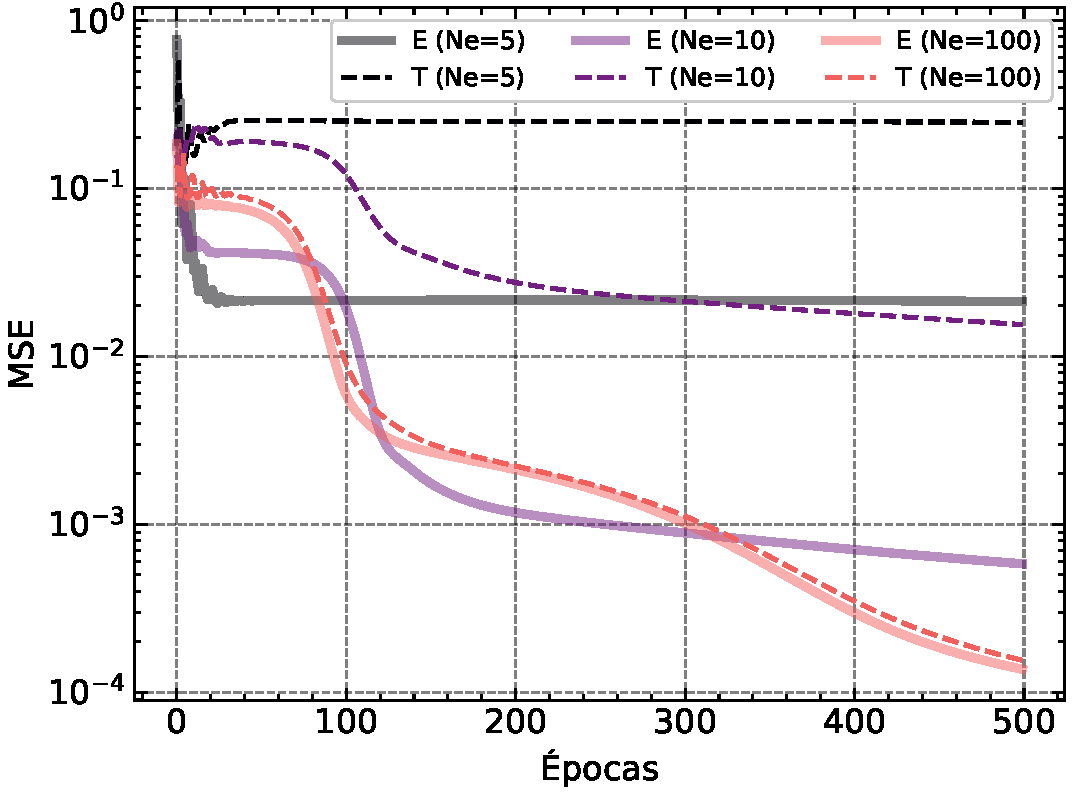
\includegraphics[width=0.45\textwidth]{figures/metrics_e3.pdf}
  \caption{métricas obtenidas durante el entrenamiento para diferentes cantidades de ejemplos de entrenamiento. E: entrenamiento, T: verificación o testing.}
  \label{fig:metrics_e3}
\end{figure}

% En la Figura \ref{fig:metrics_e3} se observa que incrementar el número de ejemplos presentados en la etapa de entrenamiento reduce el error de generalización. Es decir es más probable que se obtenga la salida correcta de algún dato que no fue presentado en el entrenamiento. En la Figura \ref{fig:predicciones_e3} se pueden ver 20 ejemplos de verificación y la salida que arroja la red.
La Figura \ref{fig:metrics_e3} muestra que aumentar el número de ejemplos en el entrenamiento reduce el error de generalización, lo que aumenta la probabilidad de obtener la salida correcta para datos no presentados durante el entrenamiento. La Figura \ref{fig:predicciones_e3} presenta 20 ejemplos de verificación y las salidas generadas por la red.

\begin{figure}
  \centering
  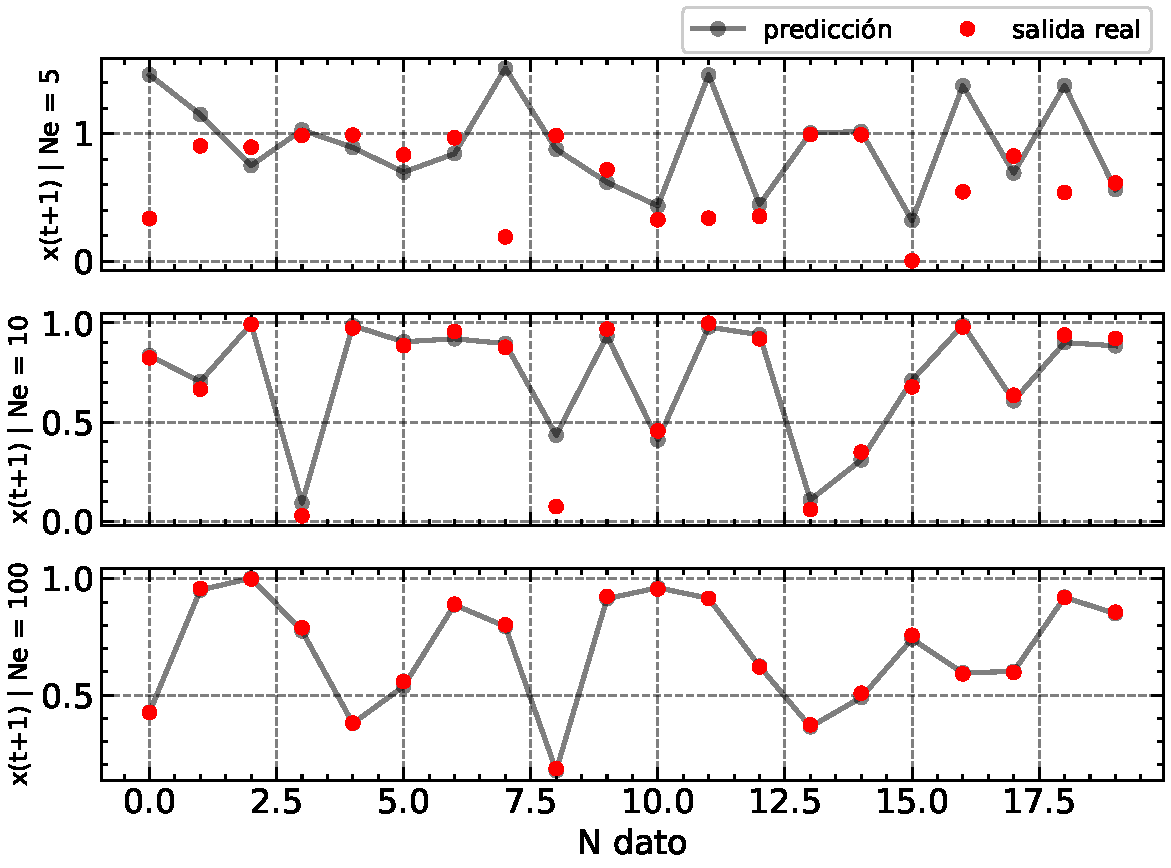
\includegraphics[width=0.45\textwidth]{figures/predicciones_e3.pdf}
  \caption{predicciones de la red luego del entrenamiento para 20 datos de entrada diferentes a los del entrenamiento. \(Ne\) indica el número de datos utilizados para el entrenamiento.}
  \label{fig:predicciones_e3}
\end{figure}

La Figura \ref{fig:predicciones_e3} confirma el comportamiento descrito anteriormente: con pocos ejemplos de entrenamiento, la red presenta un mayor error en las predicciones, pero este error disminuye a medida que aumenta la cantidad de ejemplos de entrenamiento.

\end{document}